\section{Extensions}

\subsection{Changing parameters}

To better investigate the robustness of our algorithms we tried to modify the noise increasing the standard deviation by a factor of 2. 
We noticed that, increasing the noise, the IST algoritm is less precise with respect to the DIST one, which is more robust preserving  
approximately the same success rate.

\begin{figure}[H]
    \begin{subfigure}{0.45\textwidth}
        \centering
        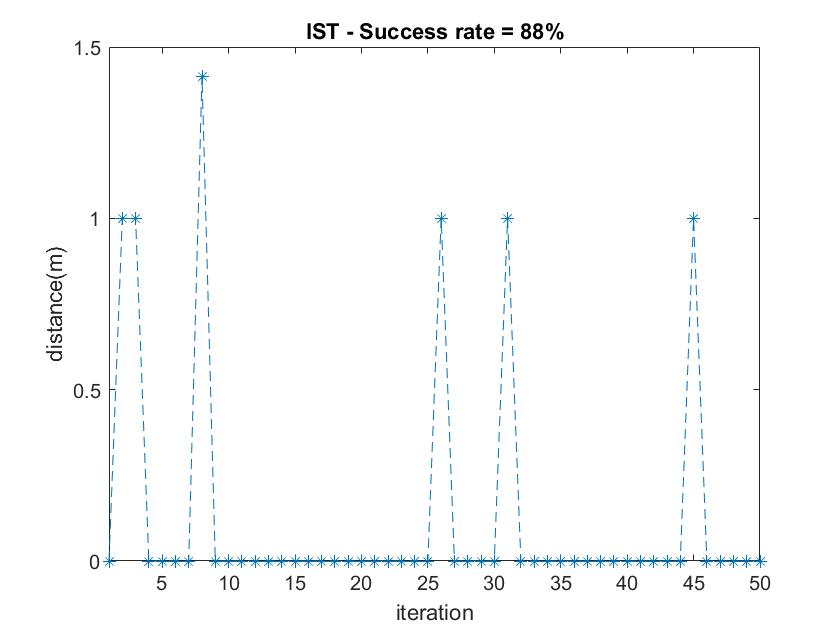
\includegraphics[width=\textwidth]{img/ist_2_devstd.jpg}
        \caption{IST}
    \end{subfigure}
    \hfill
    \begin{subfigure}{0.45\textwidth}
        \centering
        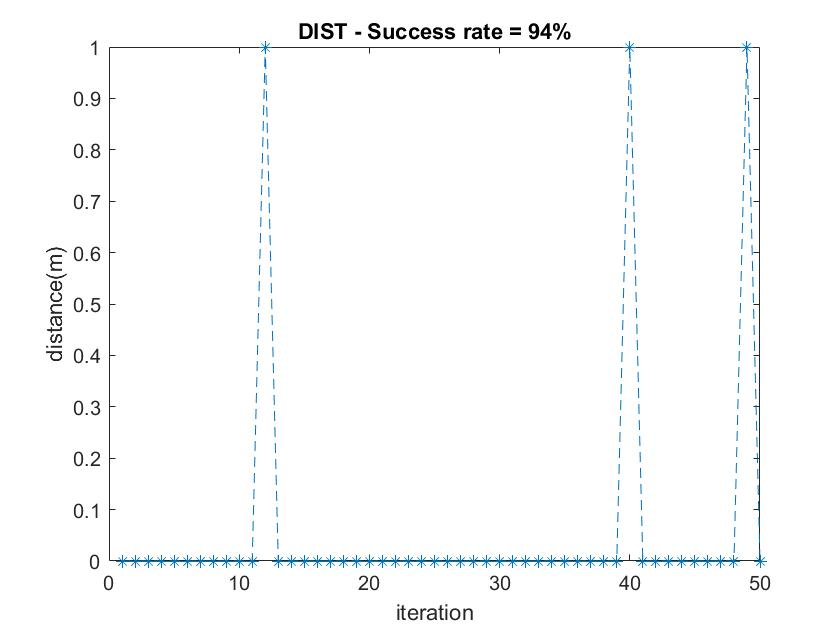
\includegraphics[width=\textwidth]{img/dist_2_devstd.jpg}
        \caption{DIST}
    \end{subfigure}
    \caption{Comparison of IST and DIST performance increasing noise}
\end{figure}

Then, we increased the number of cells from $100$ to $200$ and both the IST and DIST alghoritm performed with a very low success rate, 
due to the uniform topology, because the regions uncovered by sensors increase with the number of cells.

\begin{figure}[H]
    \begin{subfigure}{0.45\textwidth}
        \centering
        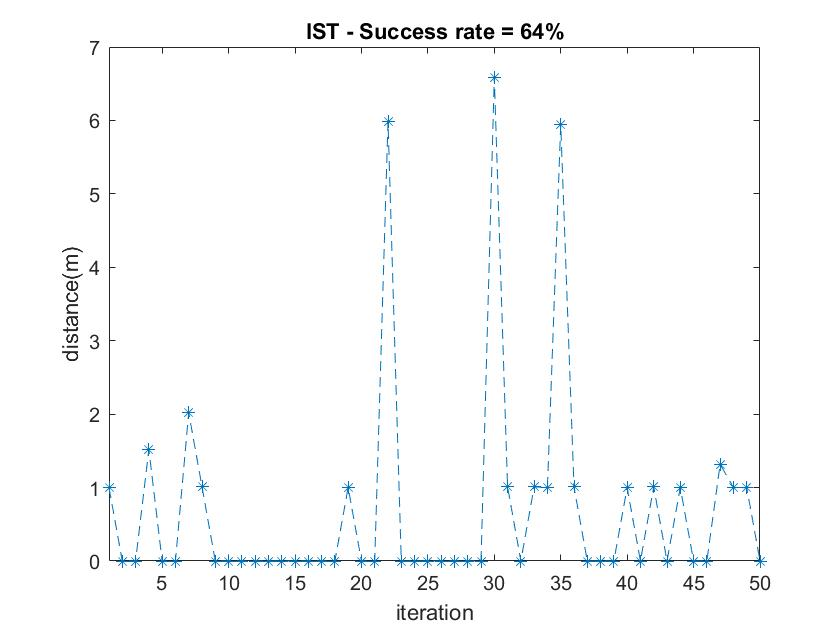
\includegraphics[width=\textwidth]{img/ist_200_p.jpg}
        \caption{IST algorithm on a grid of 200 cells}
    \end{subfigure}
    \hfill
    \begin{subfigure}{0.45\textwidth}
        \centering
        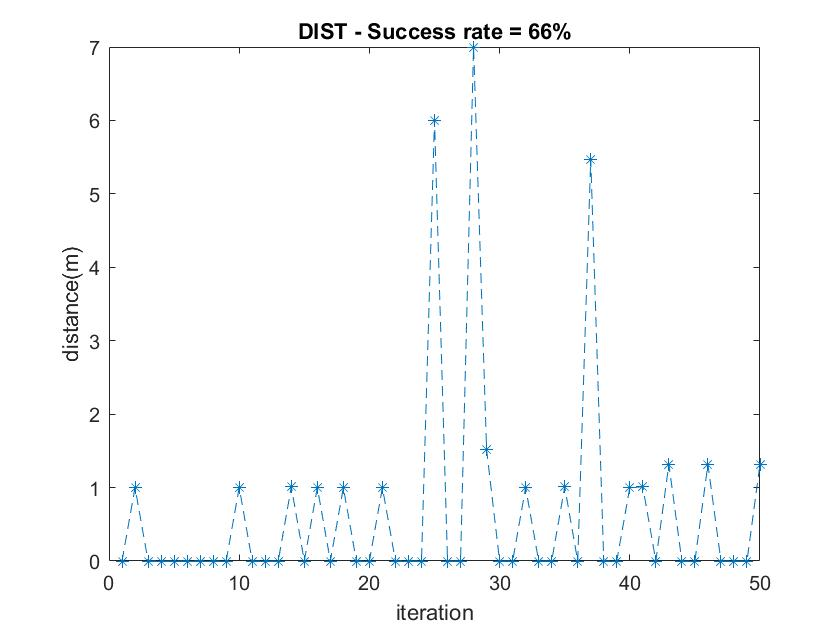
\includegraphics[width=\textwidth]{img/dist_200_p.jpg}
        \caption{DIST algorithm on a grid of 200 cells}
    \end{subfigure}
    \caption{Comparison of IST and DIST performance increasing the number of cells}
\end{figure}

We increased the number of sensors to 40 to obtain a good rate of success. After running the algorithm different times on a 
uniform topology, we empirically noticed that, to obtain a success rate of at least $80\%$, the number of sensors should be 
around $\frac{1}{4}$ or $\frac{1}{5}$ of the number of cells.

\begin{figure}[H]
    \begin{subfigure}{0.45\textwidth}
        \centering
        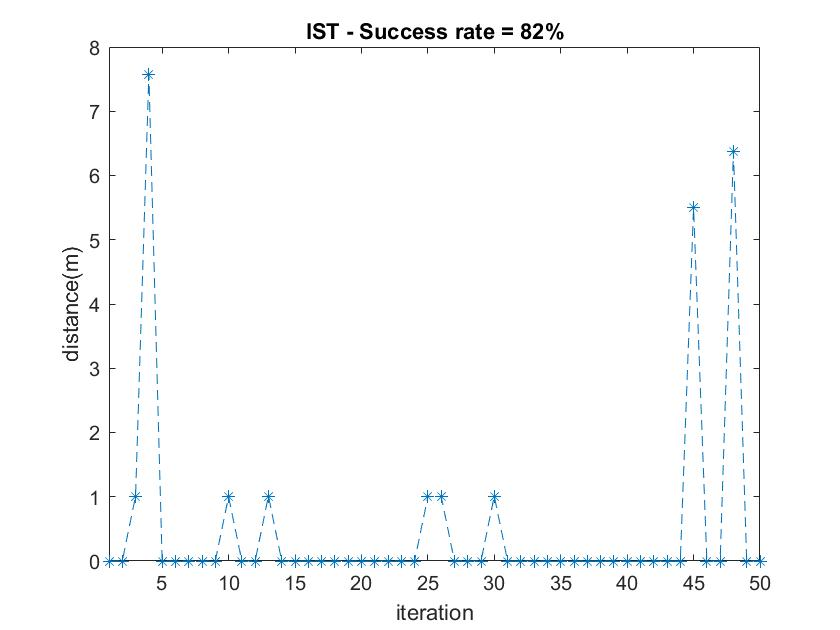
\includegraphics[width=\textwidth]{img/ist_200_p_40_n.jpg}
        \caption{IST algorithm on a grid of 200 cells and 40 sensors}
    \end{subfigure}
    \hfill
    \begin{subfigure}{0.45\textwidth}
        \centering
        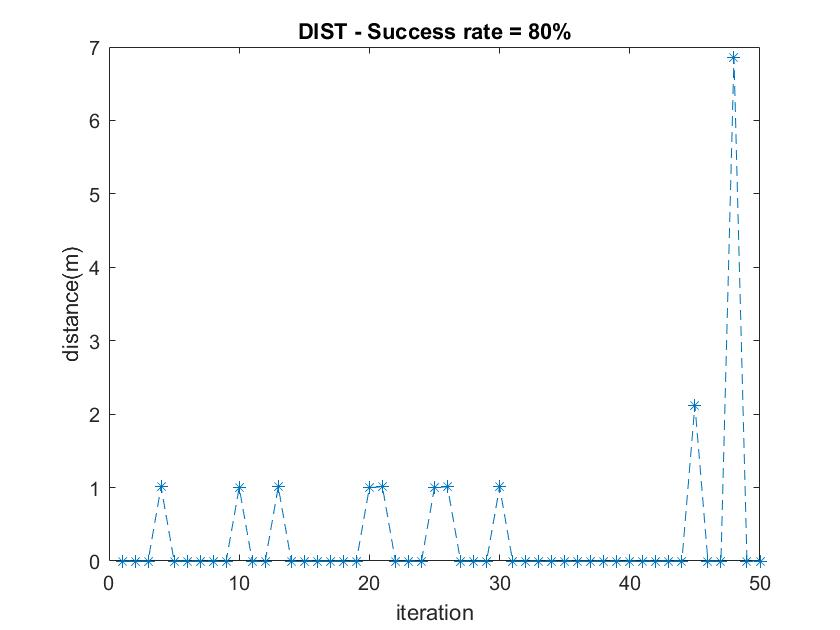
\includegraphics[width=\textwidth]{img/dist_200_p_40_n.jpg}
        \caption{DIST algorithm on a grid of 200 cells and 40 sensors}
    \end{subfigure}
    \caption{Comparison of IST and DIST performance increasing the number of cells}
\end{figure}

\subsection{k-Nearest Neighbors}

To implement the k-Nearest Neighbors algorithm we used the function \highlight{knnsearch} from the Machine Learning Toolbox. 

We noticed that, on a grid topology it rarely misses. Using a uniform topology, it's success rate is lower, but it is still very accurate ($96\%$). 
However, it is computationally intensive and the computational cost increases with the number of cells and the number of sensors.

\begin{figure}[H]
    \centering
    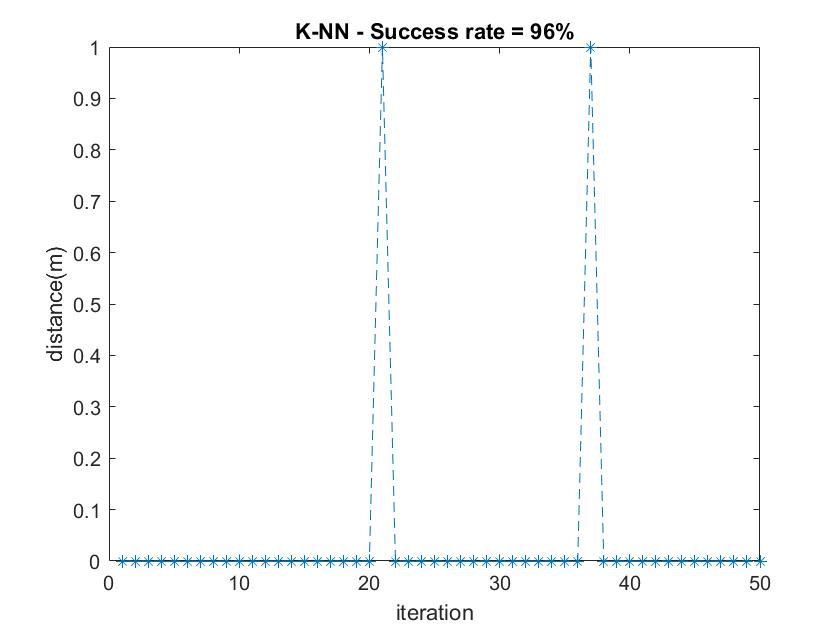
\includegraphics[width=0.45\textwidth]{img/extension_2_knn.jpg}
    \caption{k-Nearest Neighbors success rate using a uniform topology}
\end{figure}

\addtocounter{subsection}{1}

\subsection{Presence of broken sensors}
We added two broken sensors to our environment to produce a wrong \emph{RSS}. We approached to this situation as an external 
attack to the network.

We defined 
\begin{equation*}
\begin{aligned}
    B_{aug}&=\begin{bmatrix}
        A & I_n
    \end{bmatrix}\\
    z_{aug}&=\begin{bmatrix}
        x & u
    \end{bmatrix}
\end{aligned}
\quad\quad\text{with}\quad
x\in R^p,\, u\in R^n
\end{equation*}

Even if two sensors are borken, the succes rate is quite good. We also estimated the succes rate 
for the identification of the two broken sensors, which resulted to be very good ($92\%$).

\begin{figure}[H]
    \centering
    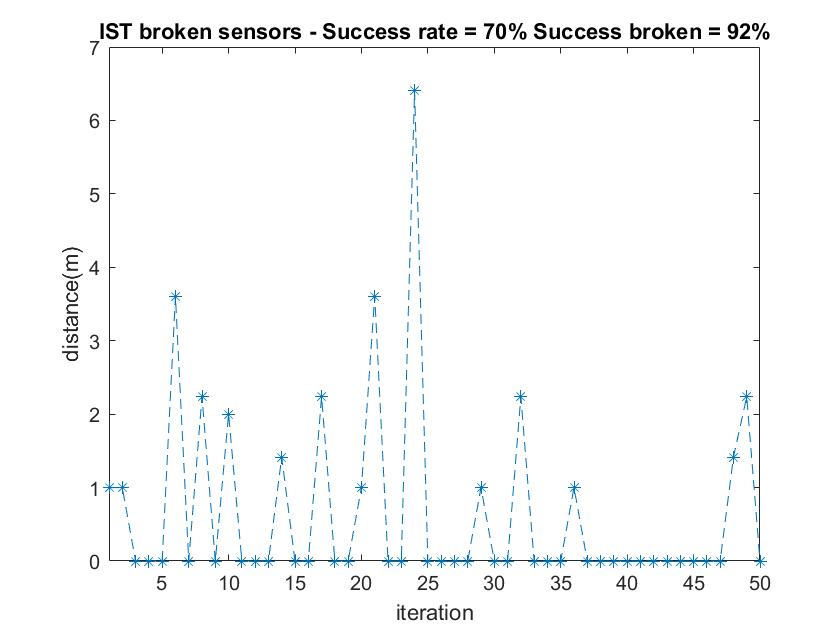
\includegraphics[width=0.45\textwidth]{img/extension_4-2.jpg}
    \caption{k-Nearest Neighbors success rate}
\end{figure}